\documentclass[11pt,a4paper]{article}
\usepackage[utf8]{inputenc}
\usepackage[margin=0.85in]{geometry}
\usepackage{amsmath,amssymb,amsthm}
\usepackage{xcolor}
\usepackage{tcolorbox}
\usepackage{graphicx}
\usepackage{booktabs}
\usepackage{array}
\usepackage{fancyhdr}
\usepackage{hyperref}
\usepackage{microtype}

% Color Palette Definitions
\definecolor{primarynavy}{RGB}{26, 54, 93}       % #1A365D - Deep Navy
\definecolor{secondaryteal}{RGB}{13, 148, 136}   % #0D9488 - Teal Accent
\definecolor{darkslate}{RGB}{45, 55, 72}        % #2D3748 - Body Text
\definecolor{lightbg}{RGB}{247, 250, 252}        % #F7FAFC - Soft Background
\definecolor{accentblue}{RGB}{49, 130, 206}      % #3182CE - Bright Blue
\definecolor{warmgold}{RGB}{214, 158, 46}        % #D69E2E - Gold Highlight
\definecolor{crimsonred}{RGB}{229, 62, 62}       % #E53E3E - Crimson Alert

\hypersetup{
    colorlinks=true,
    linkcolor=primarynavy,
    citecolor=secondaryteal,
    urlcolor=accentblue,
    pdftitle={Complete Lecture Notes: Analytical Geometry in Polar Coordinates},
    pdfauthor={Class Notes}
}

% Page Setup
\pagestyle{fancy}
\fancyhf{}
\fancyhead[L]{\small \textbf{\color{primarynavy}Analytical Geometry in Polar Coordinates (MATMJ52)}}
\fancyhead[R]{\small \textbf{\color{secondaryteal}Lectures by B.P. Sir}}
\fancyfoot[L]{\small \textcolor{primarynavy}{\href{https://www.sciqb.com}{\textbf{www.sciqb.com}}}}
\fancyfoot[C]{\thepage}
\fancyfoot[R]{\small \textcolor{secondaryteal}{\href{https://www.sciqb.com}{\textbf{SCIQB Platform}}}}
\renewcommand{\headrulewidth}{0.6pt}
\renewcommand{\footrulewidth}{0.4pt}

% Custom TColorBox Environments
\newtcolorbox{defbox}[1]{
    colback=lightbg,
    colframe=primarynavy,
    fonttitle=\bfseries\color{white},
    title={#1},
    boxrule=1pt,
    top=2.5mm, bottom=2.5mm, left=3.5mm, right=3.5mm
}

\newtcolorbox{formulabox}[1]{
    colback=secondaryteal!8!white,
    colframe=secondaryteal,
    fonttitle=\bfseries\color{white},
    title={#1},
    boxrule=1pt,
    top=2.5mm, bottom=2.5mm, left=3.5mm, right=3.5mm
}

\newtcolorbox{exbox}[1]{
    colback=white,
    colframe=accentblue,
    fonttitle=\bfseries\color{white},
    title={#1},
    boxrule=1pt,
    top=2.5mm, bottom=2.5mm, left=3.5mm, right=3.5mm
}

\setlength{\parindent}{0pt}
\setlength{\parskip}{5pt}

\begin{document}

% Title Banner
\begin{center}
    \tcbset{colframe=primarynavy,colback=primarynavy!5!white,arc=0mm}
    \begin{tcolorbox}[sharp corners, boxrule=1.5pt]
        \begin{center}
            {\Large \bfseries \color{primarynavy} MATHEMATICAL LECTURE NOTES ON ANALYTICAL GEOMETRY}\\[4pt]
            {\large \bfseries \color{secondaryteal} Polar Coordinates: Straight Line, Circle, Conic Sections, Tangents, Normals \& Chords}\\[6pt]
            {\small \textbf{Course Code:} MATMJ52 \quad|\quad \textbf{Lectures by:} B.P. Sir (07/08/2026--11/08/2026) \quad|\quad \textbf{Platform:} \href{https://www.sciqb.com}{\color{accentblue}\textbf{www.sciqb.com}}}
        \end{center}
    \end{tcolorbox}
\end{center}

\vspace{0.2cm}

\tableofcontents
\newpage

\section{Module 1: Polar Coordinates and the Polar Straight Line}

\subsection{Polar Coordinate System}

\begin{defbox}{Definition: Polar Coordinates}
Let $O$ be a fixed reference point in the plane called the \textbf{pole} (or origin), and let $OX$ be a fixed horizontal directed ray emanating from $O$ called the \textbf{initial line} (or polar axis).
\begin{itemize}
    \item \textbf{Radius Vector ($r$):} The directed distance from the pole $O$ to any point $P$, $r = |OP| \ge 0$.
    \item \textbf{Vectorial Angle ($\theta$):} The anti-clockwise angle from the initial line $OX$ to $OP$, $\theta = \angle XOP$.
\end{itemize}
The point $P$ is uniquely represented by the ordered pair $(r, \theta)$.
\end{defbox}

\begin{center}
    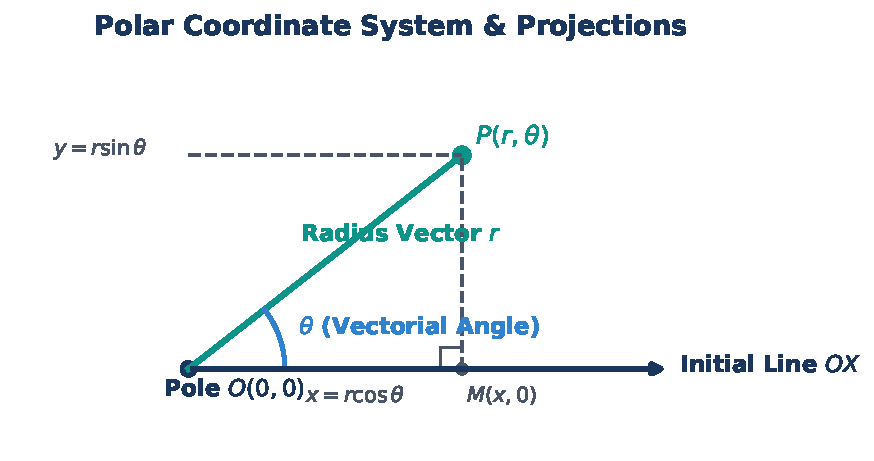
\includegraphics[width=0.72\textwidth]{figures/fig1_polar_coordinates.pdf}
\end{center}

\subsection{Polar Equation of a Straight Line}

\begin{defbox}{Theorem: Standard Polar Equation of a Straight Line}
Let $p$ be the length of the perpendicular drawn from the pole $O$ to the straight line $RS$, and let $\alpha$ be the angle that this normal $ON$ makes with the initial line $OX$. Then the polar equation of the straight line is:
\begin{equation}
    \mathbf{p = r \cos(\theta - \alpha) \iff \frac{p}{r} = \cos(\theta - \alpha)}
\end{equation}
\end{defbox}

\begin{exbox}{Step-by-Step Proof from Right Triangle $\triangle ONR$}
\begin{enumerate}
    \item Consider a straight line $RS$. Draw perpendicular $ON \perp RS$ from the pole $O$.
    \item Let $ON = p$, and let the polar coordinates of $N$ be $(p, \alpha)$, so $\angle XON = \alpha$.
    \item Let $R(r, \theta)$ be any point on $RS$, so $OR = r$ and $\angle XOR = \theta$.
    \item In the right-angled triangle $\triangle ONR$:
    \begin{equation}
        \angle NOR = \angle XOR - \angle XON = \theta - \alpha
    \end{equation}
    \item By standard right-triangle trigonometry:
    \begin{equation}
        \cos(\angle NOR) = \frac{ON}{OR} \implies \cos(\theta - \alpha) = \frac{p}{r} \implies \mathbf{p = r\cos(\theta - \alpha)}
    \end{equation}
\end{enumerate}
\end{exbox}

\begin{center}
    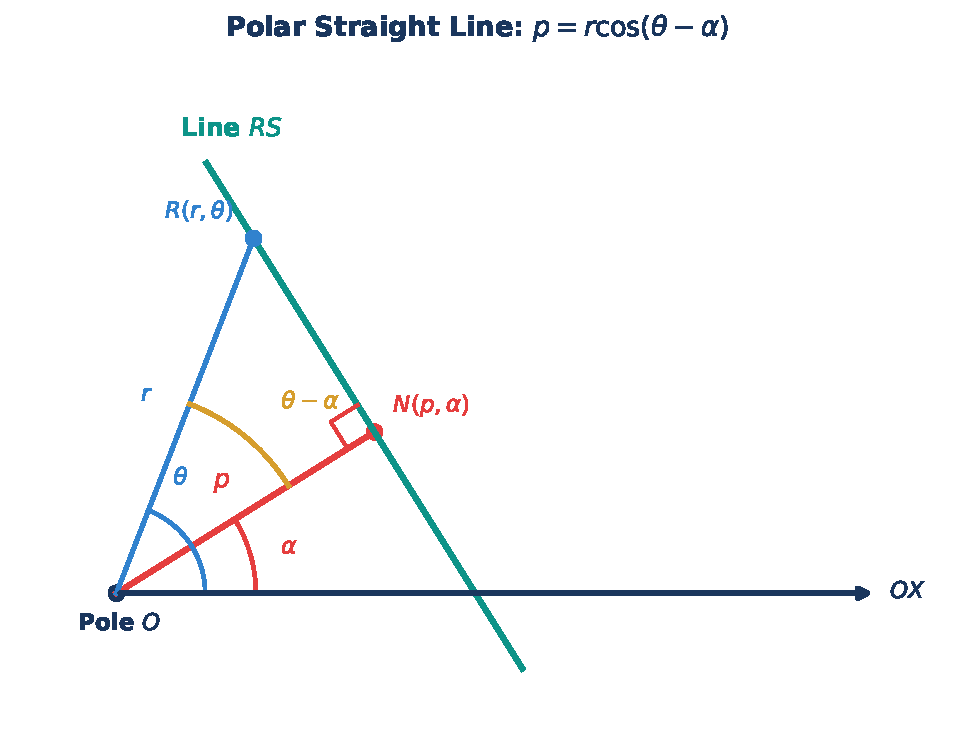
\includegraphics[width=0.75\textwidth]{figures/fig2_polar_straight_line.pdf}
\end{center}

\newpage

\subsection{Properties and Special Cases of the Polar Straight Line}

\begin{formulabox}{Important Forms and Special Cases}
\begin{enumerate}
    \item \textbf{Cartesian Form:} Expanding $p = r\cos(\theta - \alpha)$:
    \begin{equation}
        p = r(\cos\theta\cos\alpha + \sin\theta\sin\alpha) \implies \mathbf{p = x\cos\alpha + y\sin\alpha}
    \end{equation}
    
    \item \textbf{General Linear Form:}
    \begin{equation}
        \frac{p}{r} = \cos\theta\cos\alpha + \sin\theta\sin\alpha \implies \mathbf{\frac{1}{r} = A\cos\theta + B\sin\theta}
    \end{equation}
    where $A = \frac{\cos\alpha}{p}$ and $B = \frac{\sin\alpha}{p}$.
    
    \item \textbf{Line Perpendicular to Initial Line ($\alpha = 0$):}
    \begin{equation}
        p = r\cos\theta \iff x = p
    \end{equation}
    
    \item \textbf{Line Parallel to Initial Line ($\alpha = \pi/2$):}
    \begin{equation}
        p = r\cos\left(\theta - \frac{\pi}{2}\right) = r\sin\theta \iff y = p
    \end{equation}
    
    \item \textbf{Line Passing Through the Pole ($p = 0$):}
    \begin{equation}
        \cos(\theta - \alpha) = 0 \implies \mathbf{\theta = \alpha \pm \frac{\pi}{2} = \text{constant}}
    \end{equation}
    
    \item \textbf{Parallel Lines:} Two parallel lines have the form $r\cos(\theta - \alpha) = p$ and $r\cos(\theta - \alpha) = p'$.
    
    \item \textbf{Mutually Perpendicular Lines:} Two perpendicular lines have the form $r\cos(\theta - \alpha) = p$ and $r\cos(\theta - \alpha') = p'$ where $\alpha' \sim \alpha = \pi/2$, i.e., $r\sin(\theta - \alpha) = p'$.
\end{enumerate}
\end{formulabox}

\newpage

\section{Module 2: Polar Equation of a Circle}

\subsection{General Equation of a Circle}

\begin{defbox}{Theorem: General Polar Equation of a Circle}
The polar equation of a circle of radius $a$ with center at $C(R, \alpha)$ is:
\begin{equation}
    \mathbf{r^2 - 2rR\cos(\theta - \alpha) + R^2 - a^2 = 0}
\end{equation}
\end{defbox}

\begin{exbox}{Step-by-Step Proof using the Law of Cosines on $\triangle POC$}
\begin{enumerate}
    \item Let $O$ be the pole, $OX$ the initial line.
    \item Let $C(R, \alpha)$ be the center of the circle, so $OC = R$ and $\angle XOC = \alpha$.
    \item Let $P(r, \theta)$ be any point on the circle, so $OP = r$, $CP = a$ (radius), and $\angle XOP = \theta$.
    \item In triangle $\triangle POC$, the included angle is $\angle POC = \theta - \alpha$.
    \item By the Law of Cosines in $\triangle POC$:
    \begin{equation}
        CP^2 = OP^2 + OC^2 - 2(OP)(OC)\cos(\angle POC)
    \end{equation}
    \item Substituting $CP = a$, $OP = r$, $OC = R$:
    \begin{align}
        a^2 &= r^2 + R^2 - 2rR\cos(\theta - \alpha) \notag \\
        \mathbf{r^2 - 2rR\cos(\theta - \alpha) + R^2 - a^2} &= \mathbf{0}
    \end{align}
\end{enumerate}
\end{exbox}

\begin{center}
    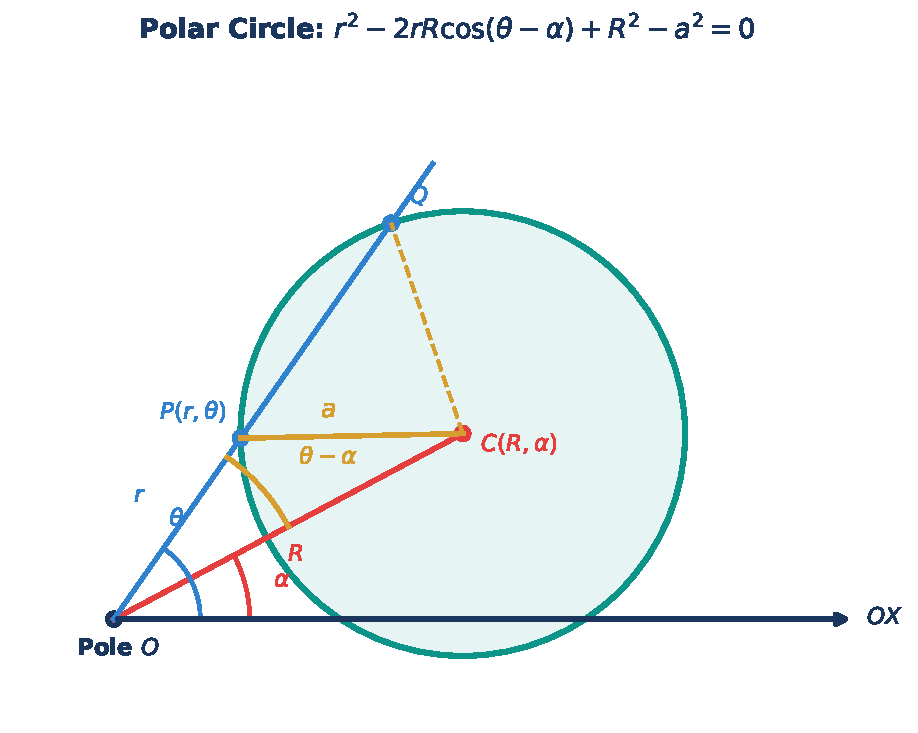
\includegraphics[width=0.75\textwidth]{figures/fig3_polar_circle_general.pdf}
\end{center}

\newpage

\subsection{Standard Particular Cases of the Polar Circle}

\begin{formulabox}{Particular Configurations of the Circle}
\begin{enumerate}
    \item \textbf{Center on Initial Line ($\alpha = 0$):}
    \begin{equation}
        r^2 - 2rR\cos\theta + R^2 - a^2 = 0
    \end{equation}
    
    \item \textbf{Pole on Circumference ($R = a$):}
    \begin{equation}
        r^2 - 2ra\cos(\theta - \alpha) = 0 \implies \mathbf{r = 2a\cos(\theta - \alpha)}
    \end{equation}
    
    \item \textbf{Pole on Circumference and Initial Line is Diameter ($\alpha = 0, R = a$):}
    \begin{equation}
        \mathbf{r = 2a\cos\theta}
    \end{equation}
    
    \item \textbf{Pole on Circumference and Initial Line is Tangent at Pole ($\alpha = \pi/2, R = a$):}
    \begin{equation}
        r = 2a\cos\left(\theta - \frac{\pi}{2}\right) \implies \mathbf{r = 2a\sin\theta}
    \end{equation}
    
    \item \textbf{Pole at Center ($R = 0$):}
    \begin{equation}
        r^2 - a^2 = 0 \implies \mathbf{r = a}
    \end{equation}
\end{enumerate}
\end{formulabox}

\begin{center}
    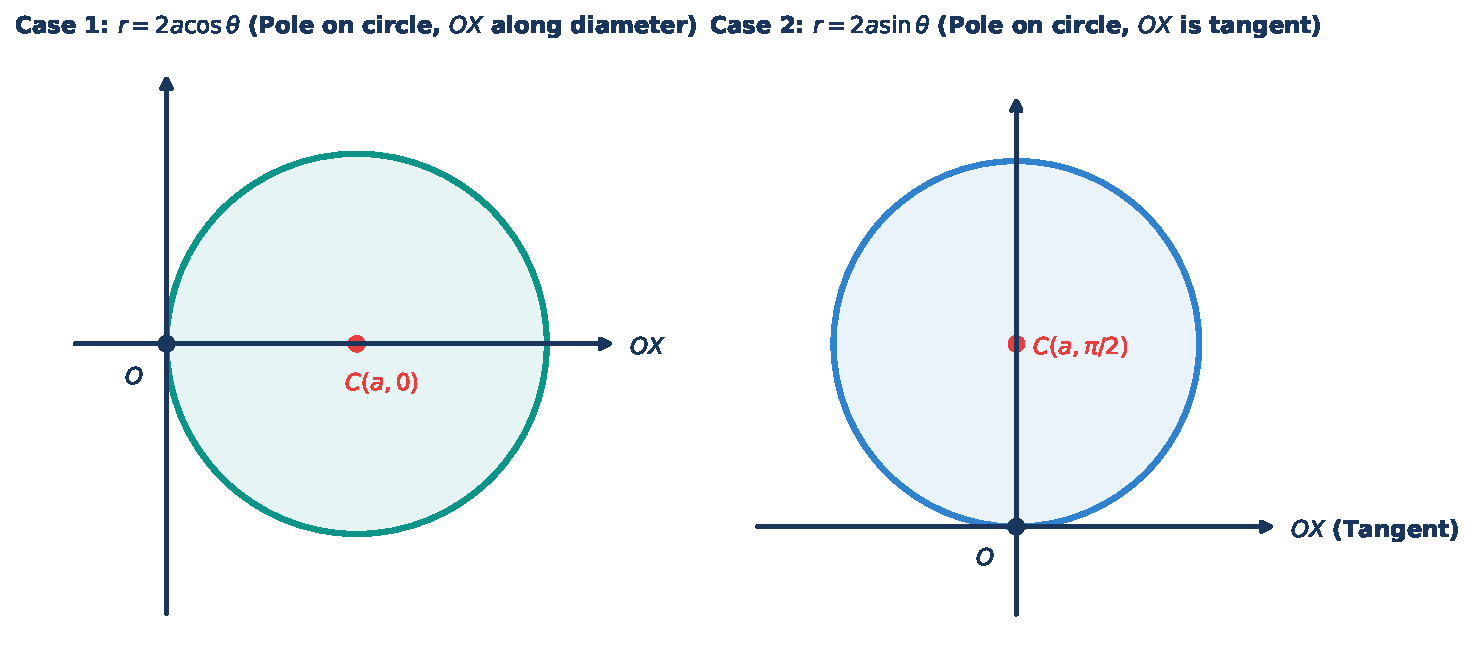
\includegraphics[width=0.92\textwidth]{figures/fig4_polar_circle_cases.pdf}
\end{center}

\newpage

\section{Module 3: Polar Equation of a Conic (Focus as Pole)}

\subsection{Standard Conic Equation \texorpdfstring{$\frac{l}{r} = 1 + e\cos\theta$}{l/r = 1 + e cos theta}}

\begin{defbox}{Theorem: Polar Equation of a Conic}
Let the focus $S$ be taken as the pole, and let $SX$ perpendicular to the directrix $XM$ be the initial line. Then the polar equation of the conic is:
\begin{equation}
    \mathbf{\frac{l}{r} = 1 + e\cos\theta}
\end{equation}
where $e$ is the eccentricity and $l$ is the semi-latus rectum.
\end{defbox}

\begin{exbox}{Step-by-Step Proof from Focus-Directrix Property}
\begin{enumerate}
    \item Let $S$ be the focus (pole), $XM$ the directrix, and $SX$ the initial line perpendicular to $XM$.
    \item Let $P(r, \theta)$ be any point on the conic. Draw $PN \perp SX$ and $PM \perp XM$.
    \item Let $SL = l$ be the semi-latus rectum ($\theta = \pi/2$).
    \item By definition of a conic: $\frac{SP}{PM} = e \implies SP = e \cdot PM$.
    \item For point $L$: $\frac{SL}{SX} = e \implies l = e \cdot SX \implies SX = \frac{l}{e}$.
    \item From the geometry of projections:
    \begin{equation}
        PM = NX = SX + SN
    \end{equation}
    \item In $\triangle SNP$: $\angle PSN = \pi - \theta$, so $SN = r\cos(\pi - \theta) = -r\cos\theta$.
    \item Therefore $PM = \frac{l}{e} - r\cos\theta$.
    \item Substituting $PM$ into $r = e \cdot PM$:
    \begin{equation}
        r = e\left(\frac{l}{e} - r\cos\theta\right) = l - er\cos\theta \implies r(1 + e\cos\theta) = l \implies \mathbf{\frac{l}{r} = 1 + e\cos\theta}
    \end{equation}
\end{enumerate}
\end{exbox}

\begin{center}
    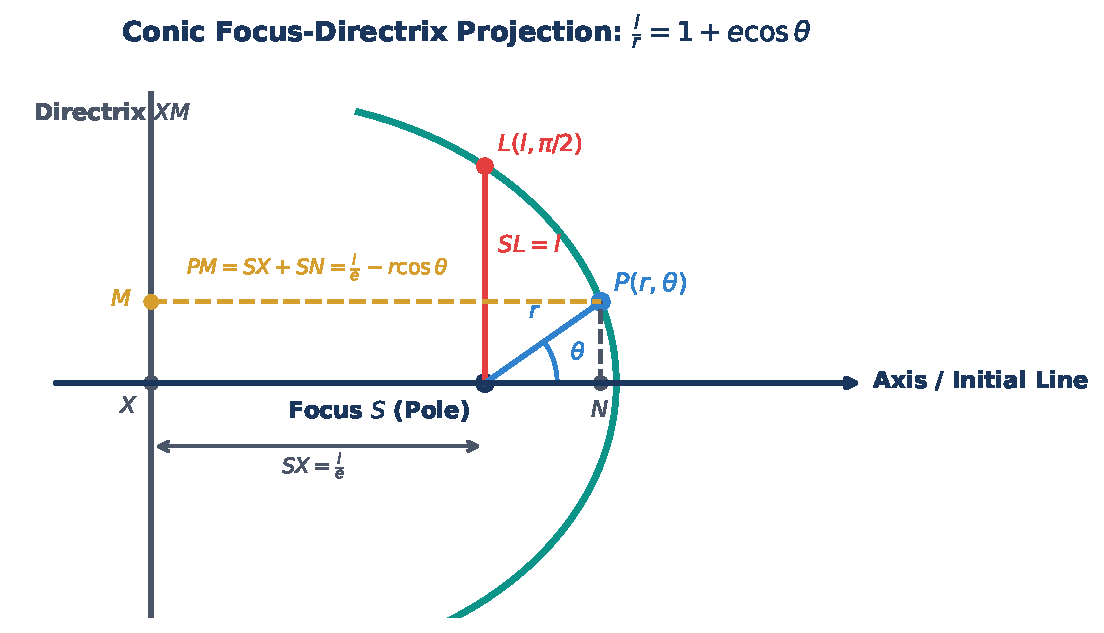
\includegraphics[width=0.82\textwidth]{figures/fig5_polar_conic_focus_directrix.pdf}
\end{center}

\newpage

\subsection{Alternative Orientations and Directrices}

\begin{formulabox}{Orientations and Directrices}
\begin{enumerate}
    \item \textbf{Axis along Negative Direction:}
    \begin{equation}
        \mathbf{\frac{l}{r} = 1 - e\cos\theta}
    \end{equation}
    
    \item \textbf{Axis Inclined at Angle $\alpha$ to Initial Line:}
    \begin{equation}
        \mathbf{\frac{l}{r} = 1 + e\cos(\theta - \alpha)}
    \end{equation}
    
    \item \textbf{Polar Equation of Directrix (Corresponding to Focus $S$):}
    \begin{equation}
        \mathbf{\frac{l}{r} = e\cos\theta}
    \end{equation}
    
    \item \textbf{Other Directrix (Central Conics):}
    \begin{equation}
        \mathbf{\frac{l}{r} = -\frac{e(1-e^2)}{1+e^2}\cos\theta}
    \end{equation}
\end{enumerate}
\end{formulabox}

\newpage

\section{Module 4: Chords, Tangents, Normals, and Chords of Contact}

\subsection{Equation of the Chord Joining Two Points}

\begin{defbox}{Theorem: Equation of Chord of a Conic}
The equation of the chord joining points $P(r_1, \alpha - \beta)$ and $Q(r_2, \alpha + \beta)$ on the conic $\frac{l}{r} = 1 + e\cos\theta$ is:
\begin{equation}
    \mathbf{\frac{l}{r} = e\cos\theta + \sec\beta \cos(\theta - \alpha)}
\end{equation}
\end{defbox}

\begin{exbox}{Step-by-Step Derivation of Chord Equation}
\begin{enumerate}
    \item Let the equation of the line $PQ$ be $\frac{l}{r} = A\cos\theta + B\sin\theta$.
    \item Since $P(\alpha - \beta)$ and $Q(\alpha + \beta)$ lie on both the conic and line:
    \begin{align}
        (A - e)\cos(\alpha - \beta) + B\sin(\alpha - \beta) &= 1 \quad \text{--- (1)} \\
        (A - e)\cos(\alpha + \beta) + B\sin(\alpha + \beta) &= 1 \quad \text{--- (2)}
    \end{align}
    \item Subtracting (1) from (2) yields $\frac{A - e}{\cos\alpha} = \frac{B}{\sin\alpha} = k$.
    \item Substituting into (1) gives $k\cos\beta = 1 \implies k = \sec\beta$.
    \item Hence $A = e + \cos\alpha\sec\beta$ and $B = \sin\alpha\sec\beta$.
    \item Substituting back into line equation:
    \begin{equation}
        \mathbf{\frac{l}{r} = e\cos\theta + \sec\beta\cos(\theta - \alpha)}
    \end{equation}
\end{enumerate}
\end{exbox}

\begin{center}
    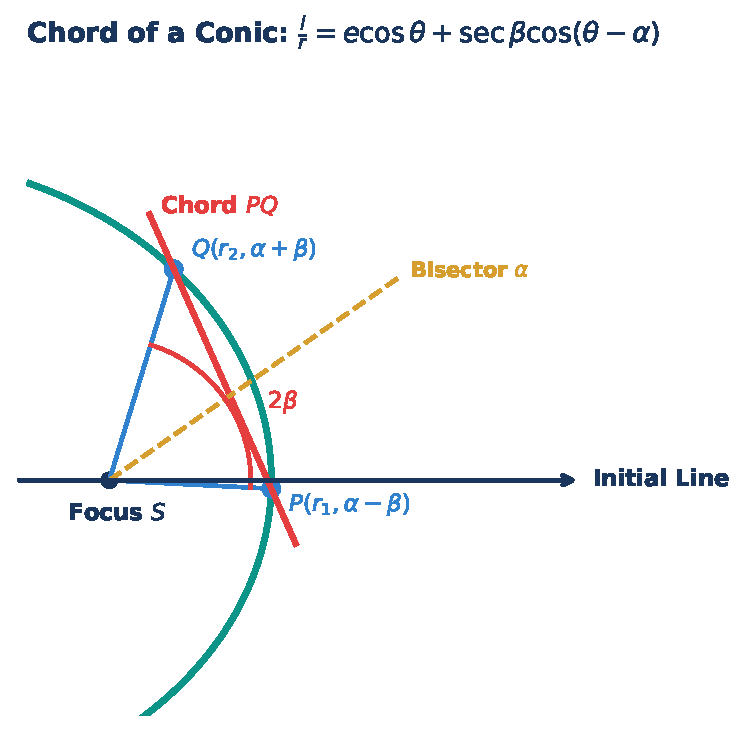
\includegraphics[width=0.75\textwidth]{figures/fig6_chord_of_conic.pdf}
\end{center}

\newpage

\subsection{Equations of Tangent and Normal}

\begin{formulabox}{Tangent and Normal to a Conic}
\begin{enumerate}
    \item \textbf{Tangent at Point $(\alpha)$ (Limiting position $\beta \to 0$):}
    \begin{equation}
        \mathbf{\frac{l}{r} = e\cos\theta + \cos(\theta - \alpha)}
    \end{equation}
    
    \item \textbf{Normal at Point of Contact $(\alpha)$:}
    \begin{equation}
        \mathbf{\frac{le\sin\alpha}{1 + e\cos\alpha} \cdot \frac{1}{r} = e\sin\theta + \sin(\theta - \alpha)}
    \end{equation}
\end{enumerate}
\end{formulabox}

\begin{center}
    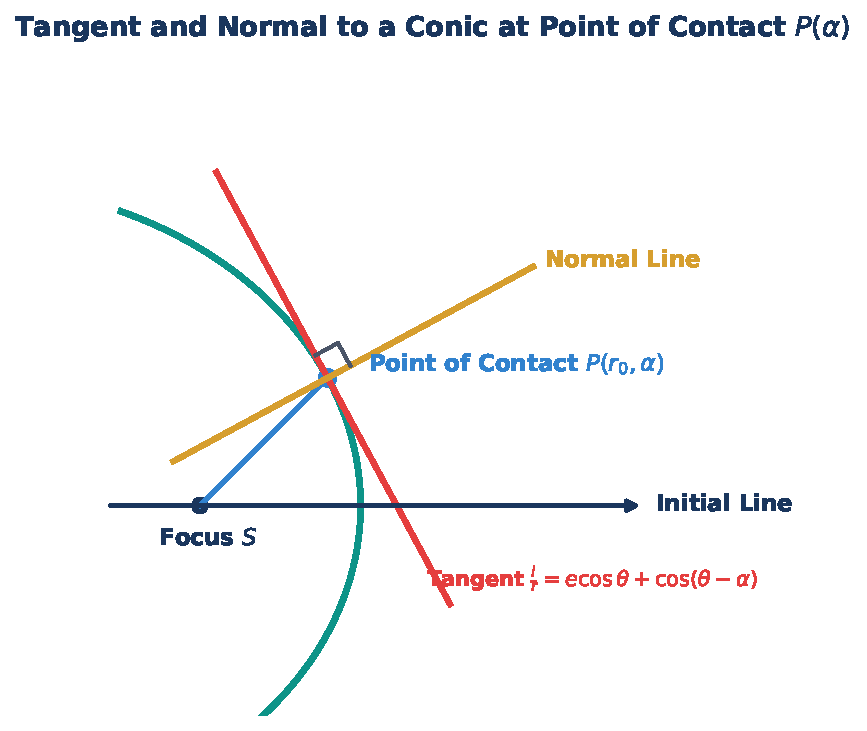
\includegraphics[width=0.75\textwidth]{figures/fig7_tangent_and_normal.pdf}
\end{center}

\newpage

\subsection{Chord of Contact of Tangents from an External Point}

\begin{defbox}{Theorem: Chord of Contact}
The chord of contact of tangents drawn from an external point $A(r_1, \theta_1)$ to the conic $\frac{l}{r} = 1 + e\cos\theta$ is:
\begin{equation}
    \mathbf{\left( \frac{l}{r} - e\cos\theta \right)\left( \frac{l}{r_1} - e\cos\theta_1 \right) = \cos(\theta - \theta_1)}
\end{equation}
\end{defbox}

\begin{exbox}{Step-by-Step Proof of Chord of Contact}
\begin{enumerate}
    \item Let tangents from $A(r_1, \theta_1)$ touch the conic at $P(\alpha - \beta)$ and $Q(\alpha + \beta)$.
    \item Equations of tangents at $P$ and $Q$ are:
    \begin{align}
        \frac{l}{r} &= e\cos\theta + \cos(\theta - \alpha + \beta) \\
        \frac{l}{r} &= e\cos\theta + \cos(\theta - \alpha - \beta)
    \end{align}
    \item Since both pass through $A(r_1, \theta_1)$:
    \begin{equation}
        \cos(\theta_1 - \alpha + \beta) = \cos(\theta_1 - \alpha - \beta) = \frac{l}{r_1} - e\cos\theta_1
    \end{equation}
    \item This gives $\alpha = \theta_1 - n\pi$ and $\sec\beta = \frac{(-1)^n}{\frac{l}{r_1} - e\cos\theta_1}$.
    \item Substituting $\alpha$ and $\sec\beta$ into the chord equation $\frac{l}{r} = e\cos\theta + \sec\beta\cos(\theta - \alpha)$:
    \begin{equation}
        \mathbf{\left( \frac{l}{r} - e\cos\theta \right)\left( \frac{l}{r_1} - e\cos\theta_1 \right) = \cos(\theta - \theta_1)}
    \end{equation}
\end{enumerate}
\end{exbox}

\begin{center}
    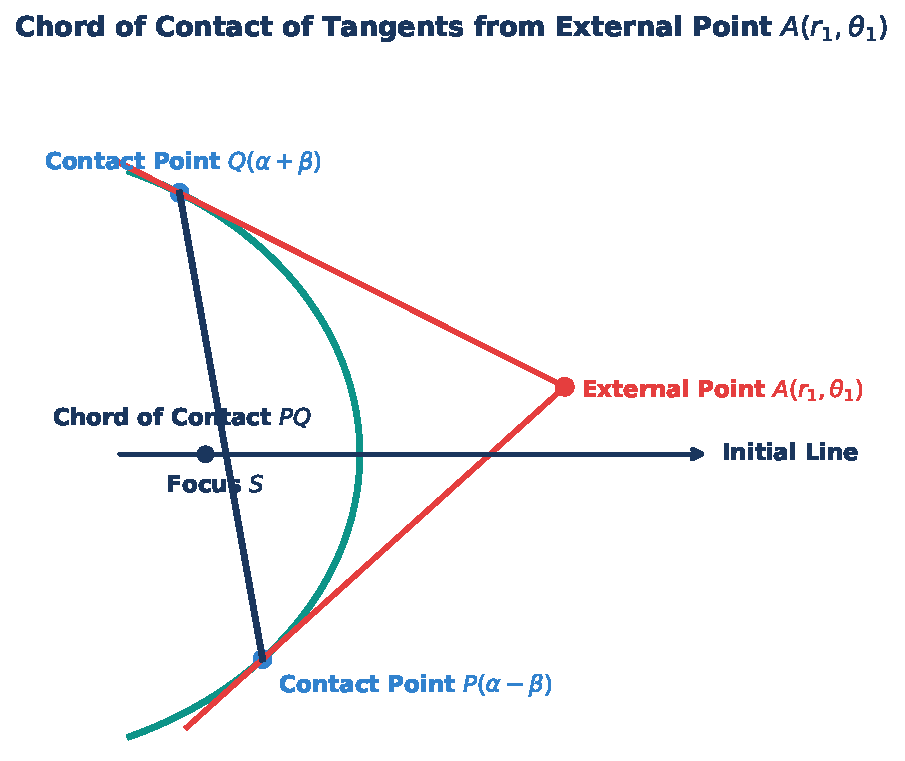
\includegraphics[width=0.78\textwidth]{figures/fig8_chord_of_contact.pdf}
\end{center}

\newpage

\section{Module 5: Fully Solved Examination Practice Problems}

\begin{exbox}{Problem 1: Determining the Nature and Parameters of a Polar Conic}
\textbf{Question:} Identify the nature, eccentricity, and semi-latus rectum of the conic given by:
\begin{equation}
    \frac{8}{r} = 4 - 5\cos\theta
\end{equation}

\textbf{Solution:}
\begin{enumerate}
    \item Divide the entire equation by $4$:
    \begin{align}
        \frac{8/4}{r} &= \frac{4}{4} - \frac{5}{4}\cos\theta \implies \mathbf{\frac{2}{r} = 1 - \frac{5}{4}\cos\theta}
    \end{align}
    \item Comparing with $\frac{l}{r} = 1 - e\cos\theta$:
    \begin{itemize}
        \item Semi-latus rectum: $\mathbf{l = 2}$
        \item Eccentricity: $\mathbf{e = \frac{5}{4} = 1.25}$
    \end{itemize}
    \item Since $e = \frac{5}{4} > 1$, the conic is a \textbf{Hyperbola}.
\end{enumerate}
\end{exbox}

\begin{exbox}{Problem 2: Finding Points on a Conic with Given Radius Vector}
\textbf{Question:} Find the points on the conic $\frac{14}{r} = 3 - 8\cos\theta$ whose radius vector is $r = 2$.

\textbf{Solution:}
\begin{enumerate}
    \item Substitute $r = 2$:
    \begin{align}
        \frac{14}{2} &= 3 - 8\cos\theta \implies 7 - 3 = -8\cos\theta \notag \\
        4 &= -8\cos\theta \implies \cos\theta = -\frac{1}{2}
    \end{align}
    \item Solving for $\theta$:
    \begin{equation}
        \cos\theta = \cos\left(\pi - \frac{\pi}{3}\right) = \cos\left(\frac{2\pi}{3}\right) \implies \theta = \pm \frac{2\pi}{3}
    \end{equation}
    \item Therefore, the required points on the conic are:
    \begin{equation}
        \mathbf{P_1 = \left(2, \frac{2\pi}{3}\right)} \qquad \text{and} \qquad \mathbf{P_2 = \left(2, -\frac{2\pi}{3}\right) \equiv \left(2, \frac{4\pi}{3}\right)}
    \end{equation}
\end{enumerate}
\end{exbox}

\newpage

\section{Module 6: Master Quick Revision Cheat Sheet}

\begin{formulabox}{1. Polar Coordinate Foundations and Distance Formulas}
\begin{itemize}
    \item \textbf{Cartesian to Polar Relations:}
    \begin{equation*}
        x = r\cos\theta, \quad y = r\sin\theta, \quad r = \sqrt{x^2 + y^2}, \quad \theta = \arctan(y/x)
    \end{equation*}
    \item \textbf{Distance Between Two Points $P_1(r_1, \theta_1)$ and $P_2(r_2, \theta_2)$:}
    \begin{equation*}
        d = \sqrt{r_1^2 + r_2^2 - 2r_1r_2\cos(\theta_1 - \theta_2)}
    \end{equation*}
    \item \textbf{Area of Triangle $\triangle OP_1P_2$ with Pole as Vertex:}
    \begin{equation*}
        \Delta = \frac{1}{2} r_1 r_2 |\sin(\theta_2 - \theta_1)|
    \end{equation*}
    \item \textbf{Collinearity of Three Points $P_1, P_2, P_3$:}
    \begin{equation*}
        \frac{\sin(\theta_2 - \theta_3)}{r_1} + \frac{\sin(\theta_3 - \theta_1)}{r_2} + \frac{\sin(\theta_1 - \theta_2)}{r_3} = 0
    \end{equation*}
\end{itemize}
\end{formulabox}

\vspace{0.2cm}

\begin{defbox}{2. Straight Lines and Circles in Polar Coordinates}
\begin{itemize}
    \item \textbf{Standard Straight Line (Normal Form):}
    \begin{equation*}
        p = r\cos(\theta - \alpha)
    \end{equation*}
    where $p$ is the length of the normal $ON$, and $\alpha$ is the inclination angle of $ON$.
    \item \textbf{General Linear Form:}
    \begin{equation*}
        \frac{1}{r} = A\cos\theta + B\sin\theta \quad \left(A = \frac{\cos\alpha}{p}, \; B = \frac{\sin\alpha}{p}\right)
    \end{equation*}
    \item \textbf{Special Straight Lines:}
    \begin{itemize}
        \item Line through pole ($p = 0$): $\theta = \text{constant}$
        \item Line perpendicular to initial line ($\alpha = 0$): $r\cos\theta = p \iff x = p$
        \item Line parallel to initial line ($\alpha = \pi/2$): $r\sin\theta = p \iff y = p$
    \end{itemize}
    \item \textbf{General Polar Circle (Center $C(R, \alpha)$, Radius $a$):}
    \begin{equation*}
        r^2 - 2rR\cos(\theta - \alpha) + R^2 - a^2 = 0
    \end{equation*}
    \item \textbf{Standard Circle Special Cases:}
    \begin{itemize}
        \item Center on initial line ($\alpha = 0$): $r^2 - 2rR\cos\theta + R^2 - a^2 = 0$
        \item Pole on circumference ($R = a$): $r = 2a\cos(\theta - \alpha)$
        \item Initial line is diameter: $r = 2a\cos\theta$
        \item Initial line is tangent at pole: $r = 2a\sin\theta$
        \item Center at pole ($R = 0$): $r = a$
    \end{itemize}
\end{itemize}
\end{defbox}

\newpage

\begin{exbox}{3. Conic Sections Referred to Focus as Pole}
\begin{itemize}
    \item \textbf{Standard Conic Equation:}
    \begin{equation*}
        \frac{l}{r} = 1 + e\cos\theta \quad \text{(Focus at pole, directrix at $x = -l/e$)}
    \end{equation*}
    \item \textbf{Conic Classification by Eccentricity $e$:}
    \begin{itemize}
        \item $e = 0 \implies$ \textbf{Circle}
        \item $0 < e < 1 \implies$ \textbf{Ellipse}
        \item $e = 1 \implies$ \textbf{Parabola}
        \item $e > 1 \implies$ \textbf{Hyperbola}
    \end{itemize}
    \item \textbf{Alternative Conic Orientations:}
    \begin{itemize}
        \item Directrix on positive side: $\frac{l}{r} = 1 - e\cos\theta$
        \item Major axis inclined at angle $\alpha$: $\frac{l}{r} = 1 + e\cos(\theta - \alpha)$
    \end{itemize}
    \item \textbf{Directrix Equations:} $\frac{l}{r} = e\cos\theta$ (corresponding directrix) and $\frac{l}{r} = -\frac{e(1-e^2)}{1+e^2}\cos\theta$ (other directrix).
    \item \textbf{Chord Joining Points $P(\alpha - \beta)$ and $Q(\alpha + \beta)$:}
    \begin{equation*}
        \frac{l}{r} = e\cos\theta + \sec\beta\cos(\theta - \alpha)
    \end{equation*}
    \item \textbf{Tangent at Point of Contact $(\alpha)$ (Limiting Case $\beta \to 0$):}
    \begin{equation*}
        \frac{l}{r} = e\cos\theta + \cos(\theta - \alpha)
    \end{equation*}
    \item \textbf{Normal at Point of Contact $(\alpha)$:}
    \begin{equation*}
        \frac{le\sin\alpha}{1 + e\cos\alpha} \cdot \frac{1}{r} = e\sin\theta + \sin(\theta - \alpha)
    \end{equation*}
    \item \textbf{Chord of Contact from External Point $A(r_1, \theta_1)$:}
    \begin{equation*}
        \left(\frac{l}{r} - e\cos\theta\right)\left(\frac{l}{r_1} - e\cos\theta_1\right) = \cos(\theta - \theta_1)
    \end{equation*}
    \item \textbf{Polar of Point $(r_1, \theta_1)$:} $\left(\frac{l}{r} - e\cos\theta\right)\left(\frac{l}{r_1} - e\cos\theta_1\right) = \cos(\theta - \theta_1)$.
\end{itemize}
\end{exbox}

\end{document}
